% !TeX root = ../tesis.tex

\chapter{Definiciones de Conceptos Fundamentales}
\label{ch:definiciones}

% =============================================================================
%  SECCIÓN 3.2 — Definición de Conceptos Fundamentales
% =============================================================================
 
\section{Definición de Conceptos Fundamentales}
\label{sec:conceptos-fundamentales}
 
El análisis de redes de transporte público desde un enfoque computacional y
matemático exige la precisión conceptual de los términos que articulan tanto el
diagnóstico del sistema como el diseño de intervenciones. En esta sección se
definen los cuatro conceptos estructurales del presente trabajo ---vulnerabilidad
urbana, planeación estratégica, eficiencia urbana e interconectividad entre
redes--- con base en la literatura especializada en teoría de grafos, redes complejas
y análisis de sistemas de movilidad. Estas definiciones no solo delimitan el alcance
teórico de la investigación, sino que también establecen los fundamentos formales
sobre los cuales se construirán los modelos computacionales, los algoritmos de
análisis y los indicadores de desempeño de la red de transporte público del área
metropolitana estudiada.

% -----------------------------------------------------------------------
\subsection{Vulnerabilidad Urbana}
\label{subsec:vulnerabilidad-urbana}
% -----------------------------------------------------------------------
 
\subsubsection{Concepto y Marco Teórico desde las Redes Complejas}
\label{subsubsec:vulnerabilidad-redes-complejas}
 
El estudio de la vulnerabilidad en sistemas de transporte urbano ha experimentado
una transición significativa: del análisis geográfico y estadístico tradicional hacia
un enfoque topológico fundamentado en la teoría de redes complejas. Este cambio
de paradigma es relevante para la presente investigación, pues permite representar
la red de transporte como un grafo matemático $\grafo = \{\nodos, \aristas\}$,
donde los nodos $\nodos$ corresponden a las estaciones y paradas, y las aristas
$\aristas$ a las rutas o conexiones entre ellas, de modo que las propiedades
estructurales globales del sistema quedan formalmente accesibles al análisis
algorítmico.
 
\textcite{loterovélez2014} señalan que una de las propiedades de mayor relevancia
práctica de las redes complejas es la capacidad del sistema para mantener algunas
de sus funciones cuando ocurren fallas, errores o ataques dirigidos a sus nodos o
vínculos; esta propiedad ha sido denominada de manera indistinta como
\termino{robustez}, \termino{resiliencia} o \termino{vulnerabilidad} por distintos
autores. En el contexto del transporte urbano, las fallas pueden corresponder a
cierres de estaciones por mantenimiento, incidentes operativos o desastres
naturales que impliquen, en términos de grafos, la eliminación de uno o varios nodos
o aristas de la red, afectando su conectividad y los flujos que la atraviesan.
 
No existe, sin embargo, un consenso único en la definición de vulnerabilidad. Según
el análisis de \textcite{loterovélez2014}, diversas corrientes han propuesto
conceptualizaciones complementarias: Holmgren (2006) la define como la
sensibilidad del sistema de infraestructura a las amenazas y perturbaciones que
puedan presentarse; Nagurney y Qiang (2011) la conciben como la cuantificación
del impacto generado por la remoción de un componente sobre el desempeño de la
red; mientras que Ouyang et al. (2009) la describen operativamente como la
disminución en la eficiencia de la red tras un ataque o falla. Para los propósitos del
presente trabajo, se adopta esta última perspectiva operativa, dado que permite
traducir el concepto de vulnerabilidad en métricas computables sobre el grafo.

\subsubsection{Fragilidad Estructural y Análisis Topológico}
\label{subsubsec:fragilidad-estructural}
 
La medición de la vulnerabilidad descansa en el análisis de las propiedades
topológicas del grafo que representa la red. \textcite{loterovélez2014} indican que
la forma más común de evaluar la robustez de una red es observar su comportamiento
después de la eliminación de uno o varios de sus elementos ---sean nodos, aristas o
una combinación de ambos---, donde dicha remoción puede ser aleatoria (simulando
una falla fortuita) o dirigida a los elementos más importantes (simulando un ataque).
 
Desde esta perspectiva, la vulnerabilidad estructural se manifiesta en el cambio de
las \termino{geodésicas} del grafo tras la perturbación. Las geodésicas, entendidas
como los caminos de menor longitud (\textit{shortest paths}) entre pares de nodos
origen-destino, constituyen el indicador central: si la eliminación de un nodo
incrementa significativamente la longitud media de dichos caminos o produce la
desconexión de componentes del grafo, ese nodo es clasificado como un punto de
fallo crítico. Albert, Jeong y Barabási (2000), citados por \textcite{loterovélez2014},
demostraron que las redes con distribución libre de escala ---caracterizadas por la
existencia de unos pocos nodos con un elevado número de conexiones, denominados
\termino{hubs}--- son robustas ante fallas aleatorias, pero altamente vulnerables ante
ataques dirigidos a dichos nodos centrales, patrón que resulta especialmente
relevante para las redes de transporte metropolitanas con nodos de alta centralidad.

Las medidas de centralidad constituyen, en consecuencia, los instrumentos
fundamentales para la identificación de nodos críticos. Según \textcite{loterovélez2014},
entre las más relevantes se encuentran: la \termino{centralidad de grado nodal}
(número de conexiones de un nodo), la \termino{centralidad de intermediación}
(proporción de caminos más cortos entre pares de nodos que pasan por el nodo en
cuestión), la \termino{centralidad de cercanía} (inverso de la suma de distancias del
nodo a los demás) y los \termino{coeficientes de cohesión} (conectividad entre los
vecinos de un nodo). En el modelo computacional que se implementa en este trabajo,
estos indicadores se calculan algorítmicamente sobre el grafo de la red para
identificar las estaciones cuya pérdida produciría el mayor impacto sistémico.

Más allá de la vulnerabilidad estructural, que considera exclusivamente la topología
del grafo, Ouyang et al. (2009), referenciados por \textcite{loterovélez2014},
distinguen una \termino{vulnerabilidad funcional} que incorpora los niveles reales de
funcionamiento de la red: frecuencias de servicio, tiempos de espera y capacidades
de carga. Esta distinción resulta crucial en el análisis de transporte público, donde la
pérdida de un nodo de alto flujo tiene consecuencias que trascienden la simple
alteración topológica y se traducen en redistribuciones de demanda sobre rutas
alternativas, potencialmente colapsando otros puntos de la red por sobrecarga.
 
Para los sistemas de transporte urbano, \textcite{loterovélez2014} afirman que una
aproximación plausible es el uso de herramientas conceptuales y analíticas de la
ciencia de la complejidad, entre ellas las redes complejas, que permiten mapear de
manera directa los elementos del sistema en nodos y vínculos. Esto fundamenta la
elección metodológica del presente trabajo: al modelar la red de transporte como un
grafo ponderado y dirigido, es posible simular computacionalmente escenarios de
falla progresiva y evaluar el comportamiento global del sistema bajo distintos niveles
de perturbación, obteniendo así un perfil de vulnerabilidad completo y cuantificado.


\begin{figure}[H]
    \centering
   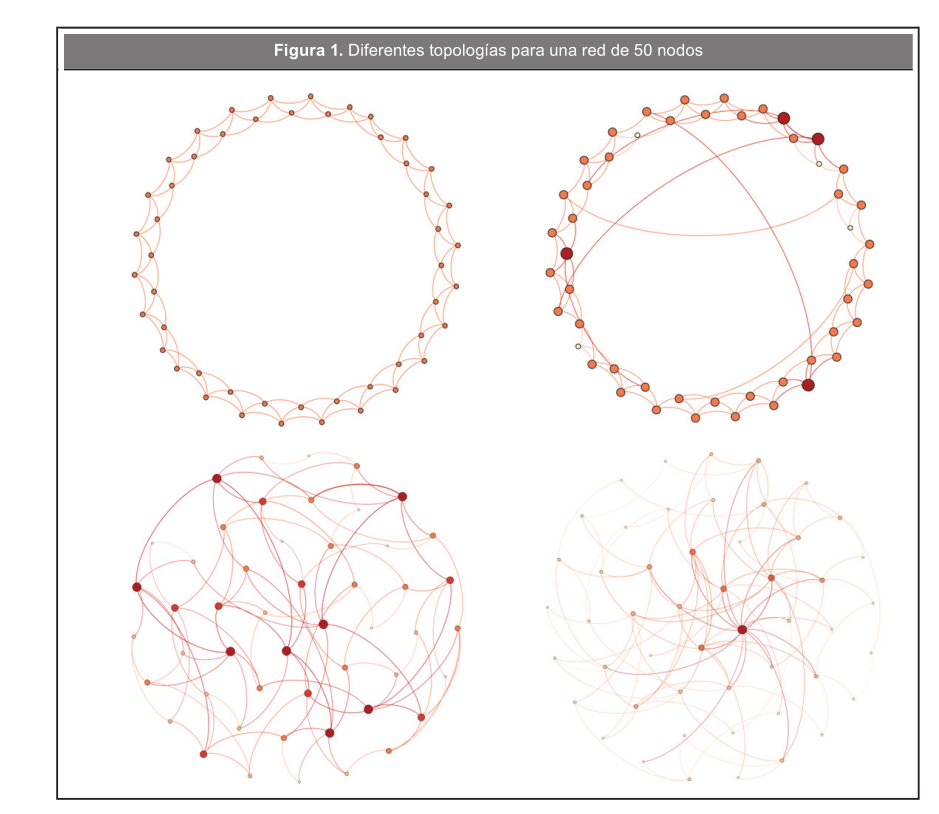
\includegraphics[width=0.90\textwidth]{Figures/Cap3/TopologiaNodos.png}
   \caption[Topologías de red y vulnerabilidad]{Cuatro topologías de red para
   50 nodos: regular, mundo pequeño, aleatoria y libre de escala.}
   \label{fig:topologias-red}
   \fuentefigura{\textcite{loterovélez2014}, p.~3.}
 \end{figure}

 % -----------------------------------------------------------------------
\subsection{Planeación Estratégica}
\label{subsec:planeacion-estrategica}
% -----------------------------------------------------------------------
 
\subsubsection{Caracterización Dinámica de la Oferta de Transporte}
\label{subsubsec:caracterizacion-dinamica}
 
La planeación estratégica del transporte público ha evolucionado de un proceso
esencialmente reactivo ---basado en la observación de demandas insatisfechas---
hacia un modelo predictivo y basado en datos que emplea el modelado computacional
de la red para anticipar los efectos de sus transformaciones. En este marco, el grafo
matemático que representa la red deja de ser un producto del análisis para
convertirse en el instrumento central de la planeación.
 
\textcite{fortin2016innovative} argumentan que, hasta la fecha de su investigación, no existía
una herramienta de análisis capaz de caracterizar sistemáticamente una red de
transporte y observar sus cambios a lo largo del tiempo de manera estructurada y
automatizada. Su propuesta aborda esta brecha mediante un método orientado a
grafos que importa datos en formato \gtfs{} (\textit{General Transit Feed
Specification}) hacia una base de datos de grafos, desde la cual se pueden calcular
algoritmos de caminos mínimos y derivar indicadores de desempeño de manera
automatizada. Este enfoque es el que adopta el presente trabajo: los datos \gtfs{}
de la red estudiada se procesan computacionalmente para construir un grafo dinámico
que refleja no solo la geometría de la red, sino también sus niveles de servicio,
frecuencias y capacidades operativas.
 
\textcite{moreno2023} refuerzan este enfoque al plantear que una metodología
robusta para la planeación requiere de una matriz origen-destino (\textsc{od}), una
red georreferenciada y los algoritmos necesarios para calcular la asignación de flujos
vehiculares. Señalan que el lenguaje Python y su ecosistema de librerías constituyen
una plataforma de reconocida eficacia para este propósito, dado que permite el
desarrollo modular del software de análisis, otorgando flexibilidad para actualizar los
modelos y extender su alcance según las necesidades de la investigación. Esta
premisa orienta directamente las decisiones de implementación tecnológica descritas
en los capítulos metodológicos posteriores.

\subsubsection{Toma de Decisiones Basada en Algoritmos y Comparación de Redes}
\label{subsubsec:comparacion-redes}
 
Una de las contribuciones más relevantes de la planeación estratégica basada en
grafos es la posibilidad de comparar cuantitativamente diferentes configuraciones de
red antes de ejecutar cambios físicos en la infraestructura.
\textcite{fortin2016innovative} proponen explícitamente la \termino{comparación de redes}
(\textit{Network Comparison}) como herramienta central de la planeación: al calcular
indicadores derivados de caminos mínimos sobre el grafo actual de la red y sobre un
grafo hipotético que incorpora modificaciones ---como la adición de nuevas líneas o
la reestructuración de rutas existentes---, es posible evaluar cuantitativamente el
impacto de cada escenario sobre el desempeño del sistema antes de tomar
decisiones de inversión.
 
Este principio resulta directamente aplicable al caso de estudio de la presente
investigación. Al modelar la red de transporte público como un grafo y simular sobre
él la incorporación del corredor anillar propuesto, los algoritmos de caminos mínimos
---como el algoritmo de \dijkstra{} o sus variantes para grafos ponderados--- permiten
cuantificar la reducción en tiempos de viaje, la mejora en la conectividad entre zonas
periféricas y la eliminación de cuellos de botella en los nodos de alta centralidad.
Así, la planeación abandona el terreno de la intuición para situarse en el de la
demostración algorítmica.
 
\textcite{moreno2023} complementan esta perspectiva al destacar que el desarrollo
modular del software de asignación permite adaptar el modelo a redes bimodales que
integren distintos modos de transporte ---como los sistemas carretera-ferrocarril o
superficie-metro--- y sus posibles intercambios a través de estaciones y puntos de
transferencia, lo que amplía significativamente el alcance analítico de la herramienta
más allá del análisis de una red monomodal.
 
\subsubsection{Enfoque en la Sostenibilidad y el Cambio Modal}
\label{subsubsec:sostenibilidad-cambio-modal}
 
La planeación estratégica del transporte público no puede disociarse de su dimensión
territorial y ambiental. \textcite{ugur2025} señalan que la integración de los
diferentes modos de transporte público ---lograda mediante la evaluación sistemática
de la conectividad entre líneas y la creación de oportunidades efectivas de
transferencia--- incrementa la cobertura espacial de la red, mejora la accesibilidad
urbana, promueve el uso del transporte colectivo y contribuye a la reducción de
emisiones, al tiempo que garantiza la equidad social en la movilidad y ofrece opciones
de viaje más económicas. Desde esta perspectiva, la planeación estratégica tiene
como objetivo último facilitar el cambio modal del vehículo privado hacia el transporte
masivo, para lo cual la optimización de la red ---modelada como grafo--- es condición
necesaria.
 
\textcite{moreno2023} enmarcan además este esfuerzo en el contexto de la soberanía
tecnológica del Estado, argumentando que el desarrollo de software propio de
asignación de tráfico, basado en herramientas de código abierto, reduce la
dependencia de licencias comerciales costosas y permite que las instituciones
públicas acumulen capacidades analíticas autónomas para la planeación del
transporte. Esta consideración es relevante para el presente trabajo, que adopta
deliberadamente una arquitectura tecnológica basada en Python y librerías de
acceso libre.

\begin{figure}[H]
   \centering
   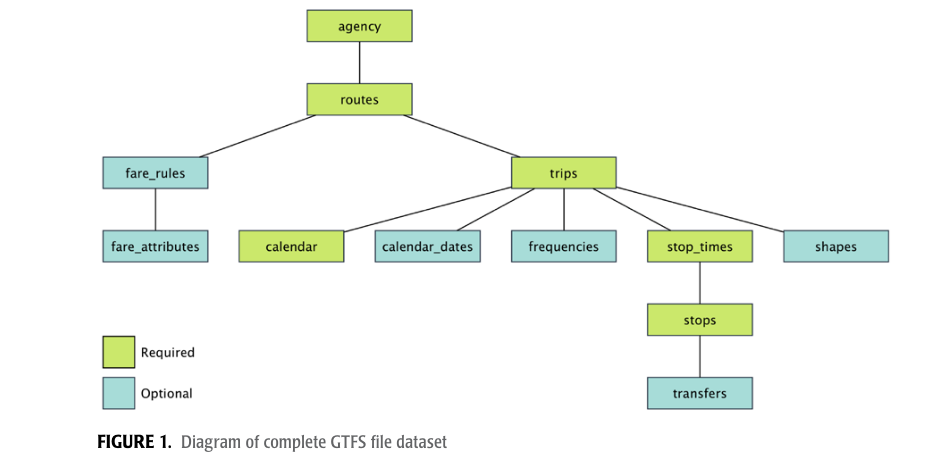
\includegraphics[width=0.85\textwidth]{Figures/Cap3/DiagramCompleteDataSetGTFS.png}
   \caption[Estructura relacional de archivos \gtfs{}]{Diagrama de la estructura
   relacional de los archivos que componen el estándar \gtfs{}.}
   \label{fig:gtfs-estructura}
   \fuentefigura{\textcite{fortin2016innovative}, p.~21.}
 \end{figure}

% -----------------------------------------------------------------------
\subsection{Eficiencia Urbana}
\label{subsec:eficiencia-urbana}
% -----------------------------------------------------------------------
 
\subsubsection{Eficiencia Topológica y Caminos Mínimos}
\label{subsubsec:eficiencia-topologica}
 
La eficiencia de una red de transporte se entiende, en su dimensión topológica, como
la capacidad del sistema para conectar cualquier par de puntos origen-destino a
través del camino de menor costo posible ---medido en términos de tiempo de viaje,
número de transbordos o distancia recorrida---. Esta propiedad es directamente
computable sobre el grafo de la red mediante algoritmos de caminos mínimos, lo que
la convierte en una de las métricas más operativas del análisis propuesto en este
trabajo.
 
\textcite{fortin2016innovative} plantean que los indicadores derivados de la teoría de grafos
---como el \termino{índice alfa} (grado de ciclicidad), el \termino{índice gamma}
(grado de conectividad) y el \termino{índice de superposición de líneas}---
caracterizan la eficiencia del diseño de la red de manera directamente relacionada
con su topología. Sin embargo, estos autores reconocen que tales indicadores no
consideran las características únicas del transporte público, como la frecuencia de
servicio, la posibilidad de transferencias entre líneas o la variabilidad del servicio a
lo largo del día; por ello proponen complementarlos con indicadores dinámicos
derivados del modelo de grafo expandido en el tiempo construido con datos \gtfs{}.
En este modelo, la eficiencia se mide a través del camino mínimo ponderado en la
dimensión temporal, que incorpora tiempos de espera y frecuencias reales de cada
línea.
 
Mishra et al. (2012), citados por \textcite{mishra2012}, introdujeron en este
contexto el concepto de \termino{índice de conectividad} de un nodo como una
medida de desempeño que va más allá de la centralidad tradicional. Este índice se
define como la suma de las potencias de conexión de todas las líneas que pasan por
un nodo, considerando características operativas como la velocidad, la capacidad, la
frecuencia, el tiempo de encabezamiento (\textit{headway}) y la distancia desde el
punto de origen. Así, la eficiencia topológica y la eficiencia operativa se integran en
una sola métrica nodal computable, que será adoptada como referencia en la
construcción de los indicadores del presente trabajo.

\subsubsection{Centralidad de Intermediación y Congestión de Rutas}
\label{subsubsec:centralidad-intermediacion}
 
La distribución de los flujos de tráfico a lo largo de la red determina, en gran medida,
su eficiencia operativa. Un sistema topológicamente bien diseñado puede resultar
ineficiente en la práctica si los flujos de demanda se concentran
desproporcionadamente sobre un subconjunto reducido de nodos o aristas, generando
congestión y tiempos de viaje superiores a los predichos por el modelo teórico.
 
\textcite{batista2015} proponen abordar este problema mediante una variación
ponderada de la \termino{centralidad de intermediación} (\textit{betweenness
centrality}), en la que el grafo de la red vial es ponderado no solo por la longitud de
las aristas, sino por el número de rutas generadas por la demanda real de tráfico,
representada mediante una matriz origen-destino (\textsc{od}). En su marco teórico,
un nodo o arista de alta centralidad de intermediación es aquel que aparece con mayor
frecuencia en los caminos mínimos entre los pares origen-destino del sistema; los
nodos con esta propiedad concentran los flujos de manera natural y son, por tanto,
los primeros en colapsar ante un incremento de demanda o una perturbación. La
eficiencia urbana aumenta cuando el sistema logra redistribuir estos flujos hacia rutas
alternativas, reduciendo la dependencia de los nodos centrales y homogeneizando
la carga sobre la red.
 
Esta perspectiva es fundamental para el análisis de la red metropolitana objeto del
presente estudio: la identificación computacional de los arcos y nodos con mayor
centralidad de intermediación ponderada por la demanda permite señalar aquellos
segmentos del sistema donde las inversiones en infraestructura o las modificaciones
de rutas producirían las mayores ganancias en eficiencia global.
 \subsubsection{Accesibilidad Espacial como Dimensión de la Eficiencia}
\label{subsubsec:accesibilidad-espacial}
 
La eficiencia urbana no se agota en la optimización interna de los flujos de la red;
incluye también la dimensión espacial de la \termino{accesibilidad}, es decir, la
capacidad del sistema de transporte para garantizar que cualquier usuario,
independientemente de su ubicación en el territorio, pueda alcanzar una cantidad
mínima de destinos dentro de umbrales de tiempo razonables.
 
\textcite{fortin2016innovative} señalan que los indicadores de accesibilidad más comunes se
calculan definiendo un radio de cobertura (por ejemplo, 500 metros como distancia
caminable aceptable) alrededor de las paradas de la red, y evaluando la proporción
de población o de empleos que quedan dentro de dicha cobertura. Sin embargo, estos
autores reconocen que este enfoque estático no incorpora la demanda real de los
usuarios ---representada por sus pares origen-destino específicos--- ni la frecuencia
del servicio, lo que limita su capacidad para reflejar la experiencia real de
accesibilidad. Proponen por ello indicadores dinámicos que, construidos sobre el
grafo ponderado en el tiempo, permiten calcular la accesibilidad real desde cualquier
nodo de la red hacia todos los demás, considerando los horarios y frecuencias del
servicio. Esta \termino{accesibilidad dinámica}, calculada algorítmicamente sobre el
modelo de grafo, constituye una medida integral de la eficiencia urbana que se
incorporará al análisis computacional de la presente investigación.

\begin{figure}[H]
   \centering
   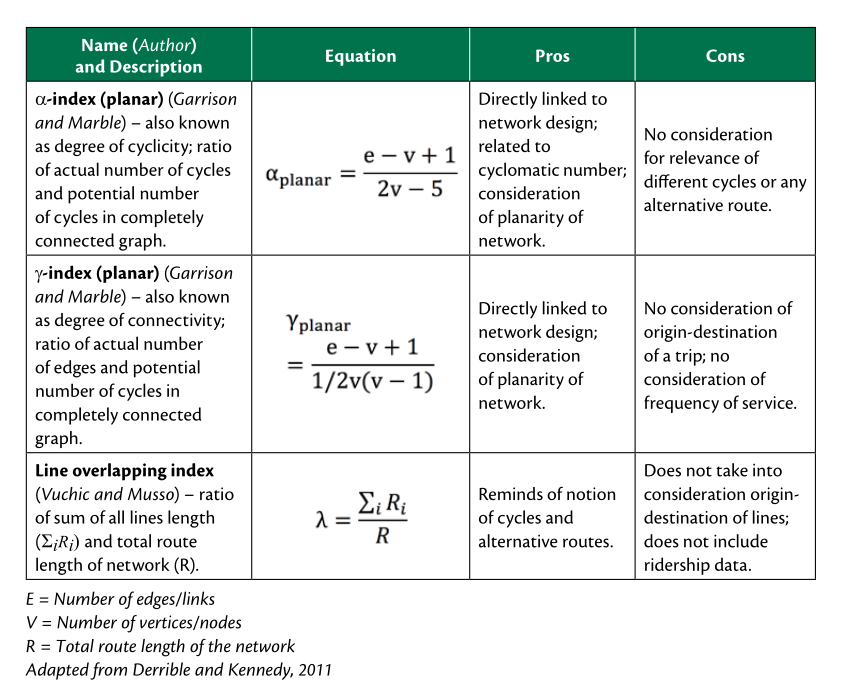
\includegraphics[width=0.85\textwidth]{Figures/Cap3/TablaIndicatorsAdaptedGraphTeory.png}
   \caption[Indices de Grafos \gtfs{}]{Tabla de indicadores de grafos \gtfs{}.}
   \label{fig:indices-grafos}
   \fuentefigura{\textcite{fortin2016innovative}, p.~23.}
 \end{figure}

% -----------------------------------------------------------------------
\subsection{Interconectividad entre Redes}
\label{subsec:interconectividad}
% -----------------------------------------------------------------------
 
\subsubsection{Integración Multimodal y Conectividad a Nivel de Nodo}
\label{subsubsec:integracion-multimodal}
 
La interconectividad entre redes es el grado en que distintos modos y líneas de
transporte público ---metro, autobús, trolebús, \brt{}, ciclovías, entre otros---
operan de manera coordinada como un sistema único y fluido, minimizando las
fricciones de la transferencia y maximizando la cobertura territorial efectiva del
sistema. En la representación por grafos, la interconectividad se modela
introduciendo \termino{aristas de transferencia} que conectan nodos de diferentes
modos o líneas dentro de un mismo grafo multimodal, con pesos que representan el
tiempo de caminata entre andenes, el tiempo de espera esperado y, en su caso, el
costo tarifario adicional del transbordo.
 
\textcite{ugur2025} afirman que la integración juega un papel crucial para garantizar
que los diferentes modos de transporte público operen de manera armoniosa,
facilitando las transferencias y permitiendo a los pasajeros desplazarse con facilidad
entre destinos. En un sistema bien integrado, la fortaleza de la conexión entre líneas
no solo amplía el área accesible para el usuario, sino que también reduce las
dificultades experimentadas durante el viaje, lo que influye positivamente en la
demanda de transporte público y contribuye a la sustitución del vehículo privado.
Su investigación sobre la línea M7 del metro de Estambul demuestra que la
evaluación sistemática de la conectividad en cada estación ---mediante un
\termino{Índice de Conectividad Simplificado} (\textsc{sci}, por sus siglas en
inglés) que incorpora variables de velocidad, capacidad de pasajeros, frecuencia,
horas de operación y distancia al origen--- revela patrones de integración desigual
que orientan directamente las decisiones de inversión y mejora operativa.

\subsubsection{Medición de la Conectividad de Parada y Penalización por Transbordo}
\label{subsubsec:penalizacion-transbordo}
 
La evaluación cuantitativa de la interconectividad requiere un índice que capture la
calidad de la conexión en cada nodo del grafo multimodal, más allá del simple conteo
de líneas que lo sirven. \textcite{mishra2012} proponen un marco de análisis basado
en la teoría de grafos que evalúa la conectividad a múltiples niveles del sistema de
transporte: el nivel de nodo (parada individual), el nivel de línea (ruta) y el nivel de
centro de transferencia (\textit{transfer center}). En este marco, el índice de
conectividad de un nodo se define como el producto de las potencias de conexión de
todas las líneas que lo atraviesan, donde la potencia de conexión de cada línea
depende de sus características operativas ---velocidad, distancia, frecuencia, tiempo
de encabezamiento, capacidad, aceleración y desaceleración--- así como de la
direccionalidad de la ruta.
 
Este enfoque supera las limitaciones de la centralidad de grado simple, que
únicamente cuenta el número de conexiones directas de un nodo sin considerar la
calidad ni la frecuencia del servicio ofrecido. \textcite{mishra2012} subrayan que
medir la conectividad puede resultar una tarea compleja y esquiva, pues es necesario
considerar tarifas, horarios, capacidad, frecuencia y otras características del sistema
en su conjunto; por ello, la evaluación de la conectividad del transporte requiere un
enfoque sistemático que integre los múltiples parámetros involucrados en la
prestación del servicio real. La diferencia entre un sistema integrado y uno
fragmentado se traduce directamente en la magnitud de la \termino{penalización por
transbordo} percibida por el usuario: cuando la conectividad en los nodos de
transferencia es alta, esta penalización se reduce, haciendo el sistema más atractivo
respecto al automóvil privado.
 
\subsubsection{El Grafo Multimodal como Marco Formal de Evaluación}
\label{subsubsec:grafo-multimodal}
 
La representación matemática de la interconectividad entre redes exige la
construcción de un \termino{grafo multimodal} en el que coexistan, sobre una misma
estructura topológica, los nodos y aristas de los distintos modos de transporte,
vinculados mediante aristas artificiales de transferencia debidamente ponderadas.
\textcite{mishra2012} señalan que, a diferencia de un enlace en una red vial ---que
es un segmento físico que conecta un nodo con otro---, un enlace en una red de
transporte público multimodal forma parte de una línea que sirve una secuencia de
paradas; dado que diferentes líneas pueden servir una misma parada, pueden existir
múltiples aristas entre los mismos nodos del grafo, lo que exige representaciones
formales más complejas que las de una red monomodal.
 
En el modelo computacional implementado en este trabajo, la red de transporte
metropolitana se representa como un grafo dirigido y ponderado
$\grafo = \{\nodos,\, \aristas,\, W\}$, donde $\nodos$ comprende el conjunto de todas
las paradas de todos los modos, $\aristas$ incluye tanto las aristas de trayecto
(intra-línea) como las aristas de transferencia (inter-modo), y $W$ es la función de
peso que asigna a cada arista un costo compuesto ---tiempo de viaje, tiempo de
espera, tiempo de caminata--- calculado a partir de los datos \gtfs{} de la red. Sobre
este grafo unificado, los algoritmos de caminos mínimos permiten evaluar la
interconectividad del sistema de manera integral: una transferencia deficiente se
traduce en un peso elevado en la arista de transbordo correspondiente, lo que el
algoritmo reflejará automáticamente como una ruta subóptima, señalando así los
nodos de transferencia que requieren intervención prioritaria.

% Sugerencia: insertar aquí el mapa de resultados SCI de Uğur y Duran (2025)
% sobre la línea M7 de Estambul, o el diagrama de grafo multimodal de Mishra
% et al. (s.f.) para la región Washington-Baltimore, una vez disponibles.
\begin{figure}[H]
  \centering
  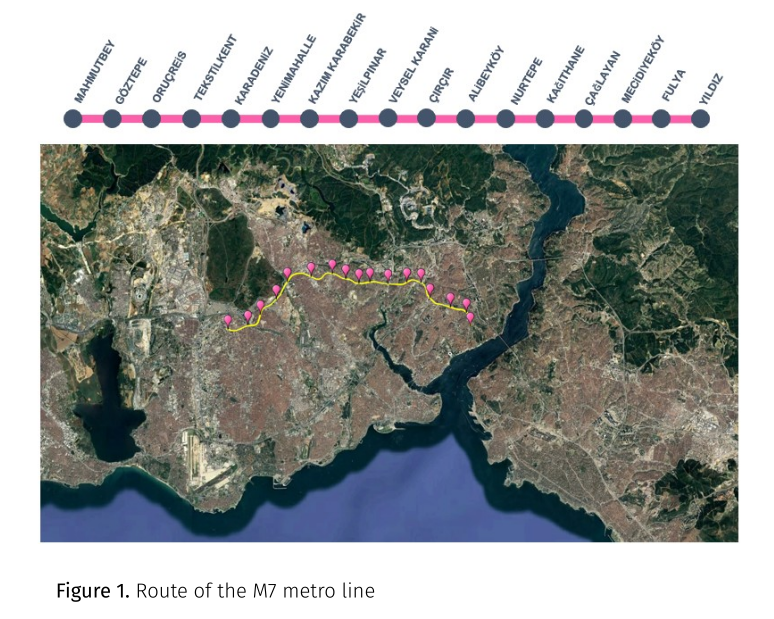
\includegraphics[width=0.88\textwidth]{Figures/Cap3/M7Estambul.png}
  \caption[Índice de Conectividad Simplificado en la línea M7 de Estambul]{
  Distribución del \textsc{sci} a lo largo de las 17 estaciones de la línea M7
  del metro de Estambul (buena, media y débil conectividad).}
  \label{fig:sci-estambul}
  \fuentefigura{\textcite{ugur2025}, p.~XX.}
 \end{figure}